\documentclass[25pt, a0paper, landscape]{tikzposter}
\tikzposterlatexaffectionproofoff

% support for LuaTeX => striclty better
%
% most things stated for LuaTeX also apply for XeTeX, but XeTeX is not
% very useful now, since LuaTeX is widely available
\usepackage{ifluatex}
\ifluatex
% use the CI font of TUM
% download from mytum portal (search for TUM CI/CD stuff)
% the scaling is the default from TUM templates
\usepackage{fontspec}
%\setsansfont{TUM Neue Helvetica}[Scale=0.95]
%\setmainfont{TUM Neue Helvetica}[Scale=0.95] % use TUM font (not a nice one)
\setmainfont{Dosis}
\usepackage{polyglossia}
\setdefaultlanguage{english}
\else
% only needed for oldschool TeX Enginge
\usepackage[utf8]{inputenc}     % does not work with LuaTeX
\usepackage[english]{babel}     % does not work well with LuaTeX
\fi

\usepackage[final]{microtype}   % improve typography, e.g. kerning



\usepackage{authblk}
\makeatletter
\renewcommand\maketitle{\AB@maketitle} % revert \maketitle to its old definition
\renewcommand\AB@affilsepx{\quad\protect\Affilfont} % put affiliations into one line
\makeatother
\renewcommand\Affilfont{\Large} % set font for affiliations

\usepackage{amsmath, amsfonts, amssymb}
\usepackage{tikz}
\usepackage{pgfplots}

% align columns of tikzposter; needs two compilations
\usepackage[colalign]{column_aligned}

% tikzposter meta settings
% \usetheme{Default}
% \usetitlestyle{Default}
% \useblockstyle{Default}
\usetheme{Simple}

\definetitlestyle{Team9Title}{
    width=600mm, roundedcorners=30, linewidth=0.4cm, innersep=1cm,
    titletotopverticalspace=15mm, titletoblockverticalspace=20mm,
    titlegraphictotitledistance=10pt, titletextscale=1
}{
    \begin{scope}[line width=\titlelinewidth, rounded corners=\titleroundedcorners]
        \draw[draw=none, fill=titlebgcolor]%
        (\titleposleft,\titleposbottom) rectangle (\titleposright,\titlepostop);
    \end{scope}
}

\usetitlestyle{Team9Title}


\defineblockstyle{Team9Blocks}{
    titlewidthscale=1, bodywidthscale=1, titleleft,
    titleoffsetx=0pt, titleoffsety=0pt, bodyoffsetx=0pt, bodyoffsety=0pt,
    bodyverticalshift=0pt, roundedcorners=0, linewidth=0.2cm,
    titleinnersep=1cm, bodyinnersep=1cm
}{
    \begin{scope}[line width=\blocklinewidth, rounded corners=\blockroundedcorners]
      % \draw[draw=framecolor]%, fill=blockbodybgcolor]
      % (blockbody.south west) rectangle (blocktitle.north east);      
      \draw[draw=framecolor]
        (blockbody.south west) rectangle (blockbody.north east);
      \ifBlockHasTitle %
           \draw[color=blocktitlebgcolor]
               (blocktitle.south west) -- (blocktitle.south east);%
       \else
        \fi
    \end{scope}
}

\useblockstyle{Team9Blocks}

% color handling
\definecolor{TumBlue}{cmyk}{1,0.43,0,0}
\colorlet{blocktitlebgcolor}{TumBlue!50}
\colorlet{blocktitlefgcolor}{TumBlue}
\colorlet{blockbodybgcolor}{TumBlue!50}
\colorlet{framecolor}{TumBlue!50}
\colorlet{backgroundcolor}{white}

\colorlet{titlebgcolor}{TumBlue}
%\colorlet{titlebgcolor}{}


%%%%%%%%%%% redefine title matter to include one logo on each side of the title; adjust with \LogoSep
\makeatletter
\newcommand\insertlogoi[2][]{\def\@insertlogoi{\includegraphics[#1]{#2}}}
\newcommand\insertlogoii[2][]{\def\@insertlogoii{\includegraphics[#1]{#2}}}
\newlength\LogoSep
\setlength\LogoSep{-70pt}

\renewcommand\maketitle[1][]{  % #1 keys
    \normalsize
    \setkeys{title}{#1}
    % Title dummy to get title height
    \node[inner sep=\TP@titleinnersep, line width=\TP@titlelinewidth, anchor=north, minimum width=\TP@visibletextwidth-2\TP@titleinnersep]
    (TP@title) at ($(0, 0.5\textheight-\TP@titletotopverticalspace)$) {\parbox{\TP@titlewidth-2\TP@titleinnersep}{\TP@maketitle}};
    \draw let \p1 = ($(TP@title.north)-(TP@title.south)$) in node {
        \setlength{\TP@titleheight}{\y1}
        \setlength{\titleheight}{\y1}
        \global\TP@titleheight=\TP@titleheight
        \global\titleheight=\titleheight
    };

    % Compute title position
    \setlength{\titleposleft}{-0.5\titlewidth}
    \setlength{\titleposright}{\titleposleft+\titlewidth}
    \setlength{\titlepostop}{0.5\textheight-\TP@titletotopverticalspace}
    \setlength{\titleposbottom}{\titlepostop-\titleheight}

    % Title style (background)
    \TP@titlestyle

    % Title node
    \node[inner sep=\TP@titleinnersep, line width=\TP@titlelinewidth, anchor=north, minimum width=\TP@visibletextwidth-2\TP@titleinnersep]
    at (0,0.5\textheight-\TP@titletotopverticalspace)
    (title)
    {\parbox{\TP@titlewidth-2\TP@titleinnersep}{\TP@maketitle}};

    \node[inner sep=0pt,anchor=west] 
    at ([xshift=-\LogoSep]title.west)
    {\@insertlogoi};

    \node[inner sep=0pt,anchor=east] 
    at ([xshift=\LogoSep]title.east)
    {\@insertlogoii};

    % Settings for blocks
    \normalsize
    \setlength{\TP@blocktop}{\titleposbottom-\TP@titletoblockverticalspace}
}
\makeatother
%%%%%%%%%%%%%%%%%%%%%%%%%%%%%%%%%%%%%


% graphics
\graphicspath{{../logs/results/}}


% title matter
\title{Image Super--Resolution with GANs}

\author[1]{Nathanael Bosch}
\author[1]{Thomas Grassinger}
\author[1]{Jonas Kipfstuhl}
\author[1]{Pierre Springer}

% remove the ugly 'and' before last author, as a benefit Pierre is in line again
\renewcommand{\Authands}{, }

% define a length for the heigt of the images
\newlength{\imageheight}
\setlength{\imageheight}{16cm}

\affil[1]{Technical University of Munich}

\insertlogoi[width=15cm]{tum_logo}
\insertlogoii[width=15cm]{tum_logo}


% main document
\begin{document}

\maketitle

\begin{columns}
  
  % Introduction and explanation of GANs
  \column{0.4}

  \block{Introduction}{%
    Some sentences about the whole project
  }
  
  \block{GANs}{%
    Maybe a picture to illustrate the idea of GANs.
  }

  % our results
  \column{0.6}

  % divide for plots and images
  \begin{subcolumns}
    % plots column
    \subcolumn{0.5}
    \block{Statistics}{%
      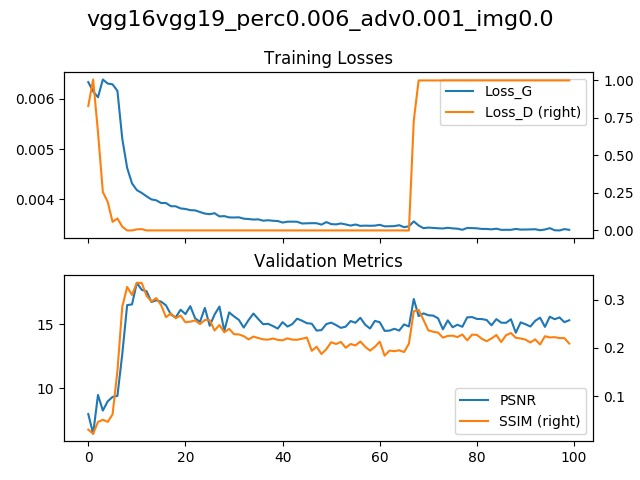
\includegraphics[width=\linewidth, height=\imageheight, keepaspectratio]{vgg16cgg19stats.jpeg}%
      % Some plots for clarifying the performance and distinguishing different Network models, e.\,g., VGG16, VGG19.
    }

    \subcolumn{0.5}
    \block{Results}{%
      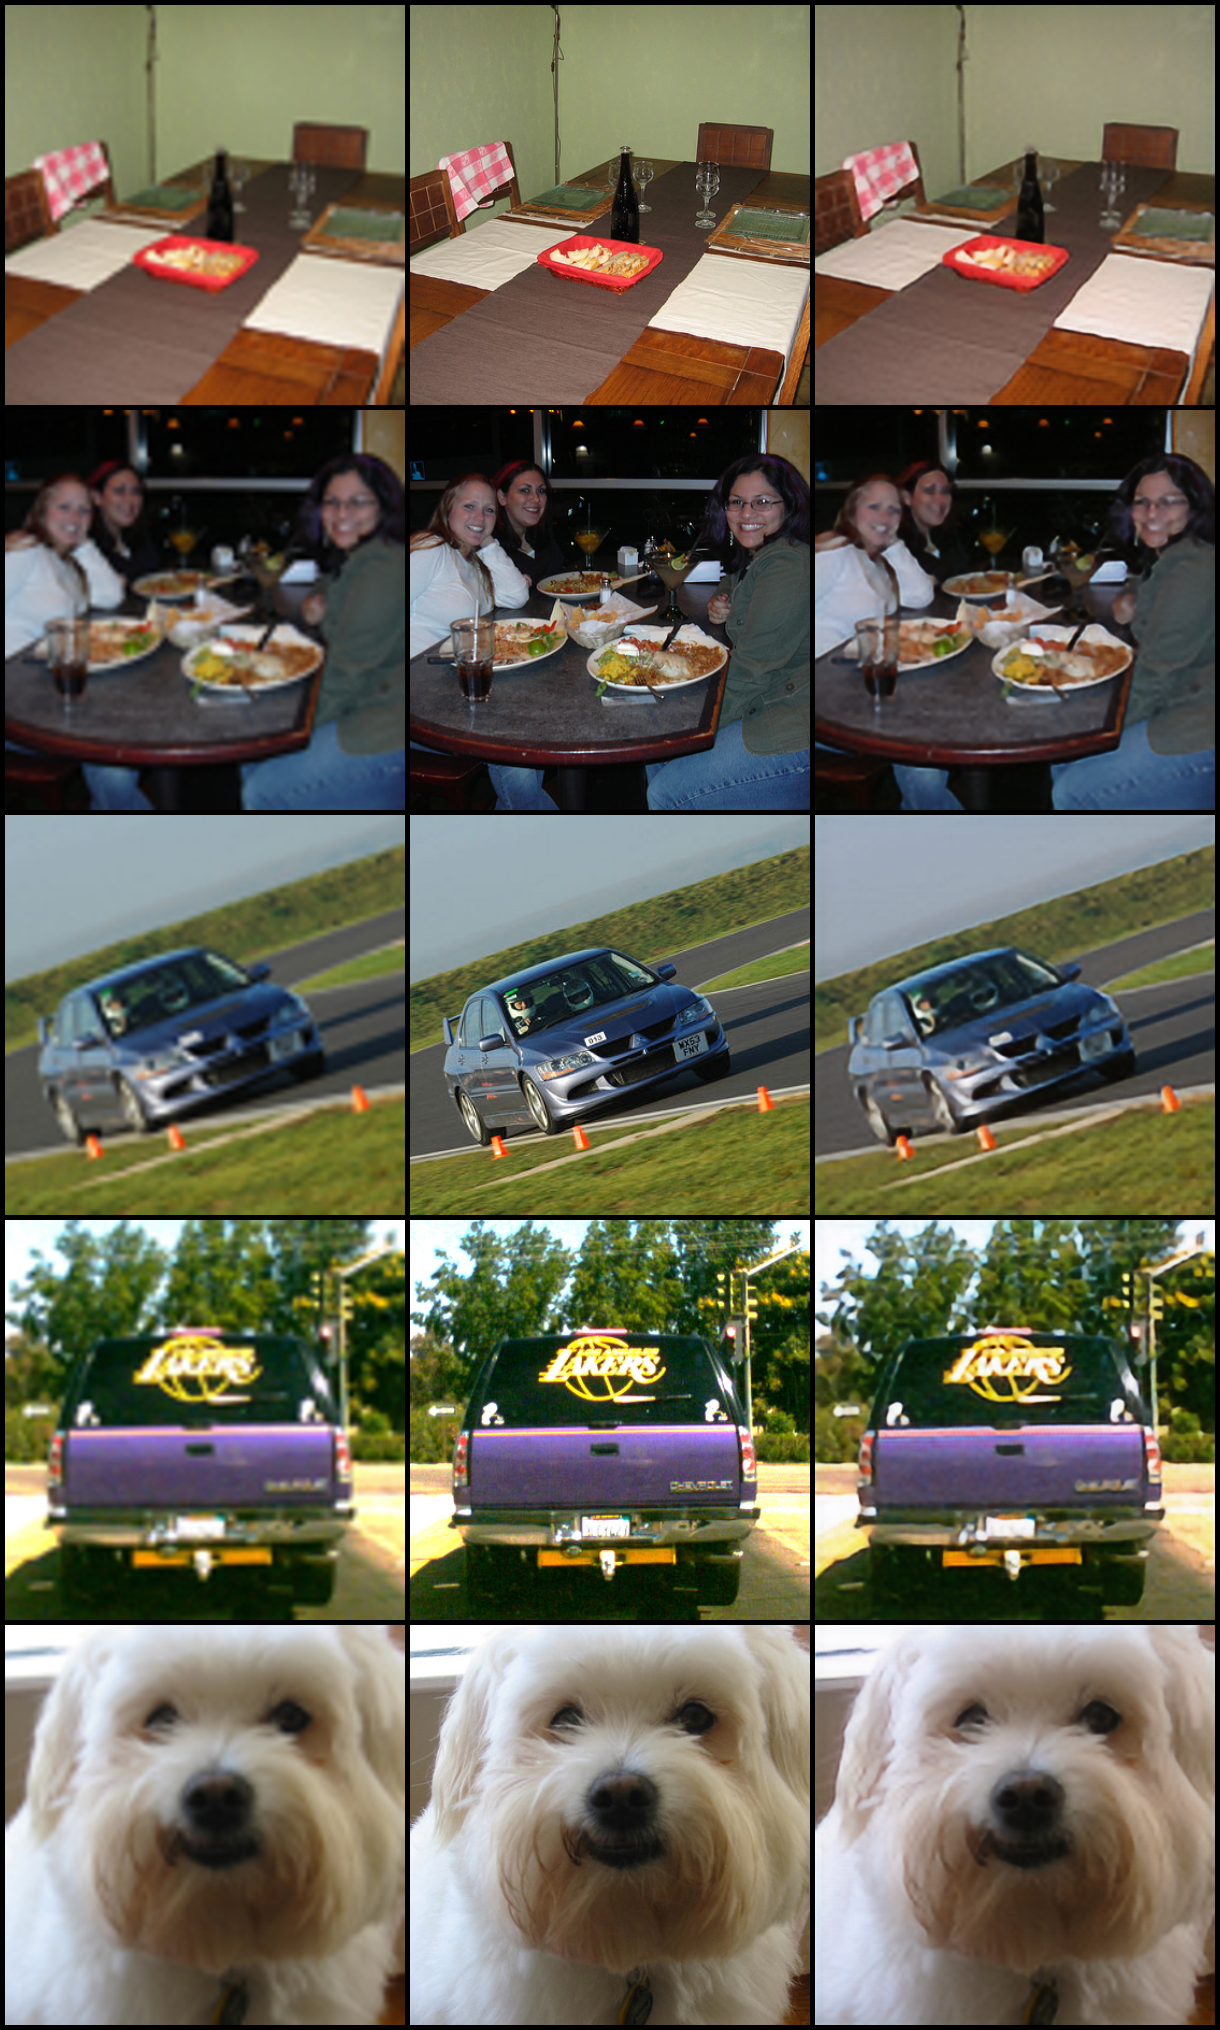
\includegraphics[width=\linewidth, height=\imageheight, clip, keepaspectratio]{epoch_11_index_10.png}%
      % Some sample images, low resultion, upsampled by our net(s), original high resolution.
    }
  \end{subcolumns}

  \begin{subcolumns}
    \subcolumn{0.5}
    \block{Statistics2}{%
      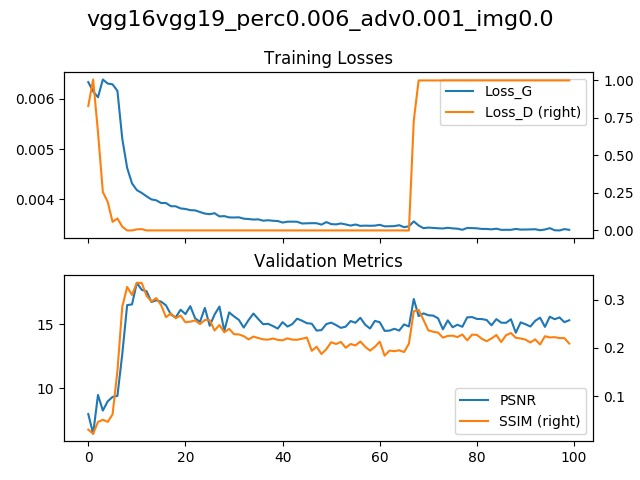
\includegraphics[width=\linewidth, height=\imageheight, keepaspectratio]{vgg16cgg19stats.jpeg}%
      % Some plots for clarifying the performance and distinguishing different Network models, e.\,g., VGG16, VGG19.
    }
    
    % images column
    \subcolumn{0.5}
    \block{Results2}{%
      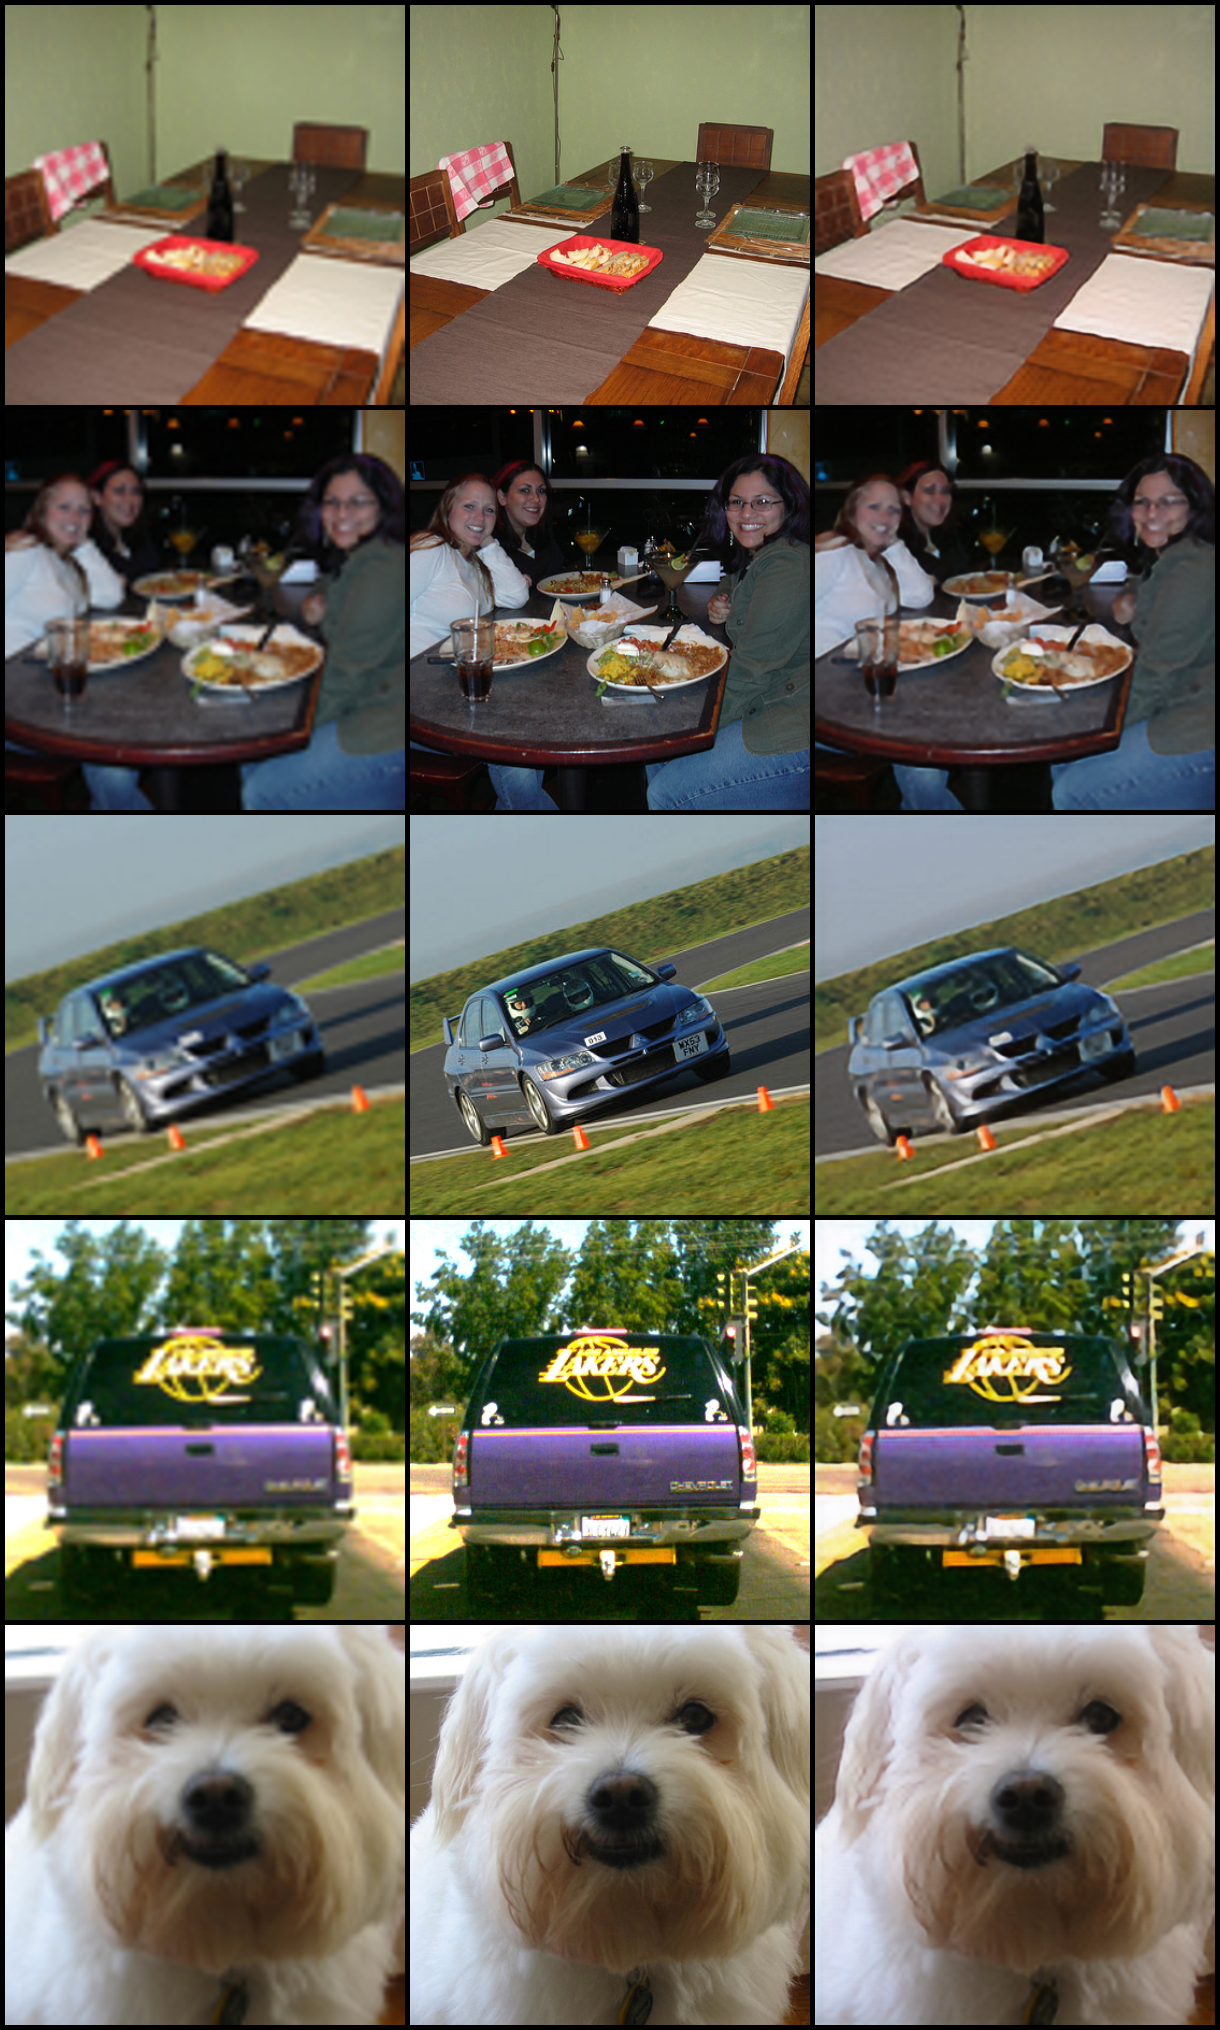
\includegraphics[width=\linewidth, height=\imageheight, clip, keepaspectratio]{epoch_11_index_10.png}%
      % Some sample images, low resultion, upsampled by our net(s), original high resolution.
    }
    
  \end{subcolumns}
  % now the keypoints of our project
  
  \block[]{Main Results}{%
    \begin{itemize}
    \item Networks learn even without discriminator
    \item Seemingly the training is faster with the use of a
      discriminator.
    \item Metrics do not change significantly after some training but
      the images get better
    \item In some settings the discriminator ``dies'' but images still
      improve
    \item Discriminator loss is extreme, either very low or very
      large; the transition is rapid
    \item Training the networks is tricky, discriminator ``dies''
      often
    \item Visually the images change very much at beginning of
      training
    \item The visual perception of the images changes for a long
      training time. Details added at late stages make the images seem
      more like actual photographs.
    \item We could not see the large jumps for the discriminator that
      was shown in the paper.
    \end{itemize}
  }


  
\end{columns}

\end{document}
